\documentclass[tikz]{standalone}

\usetikzlibrary{shapes}

\begin{document}
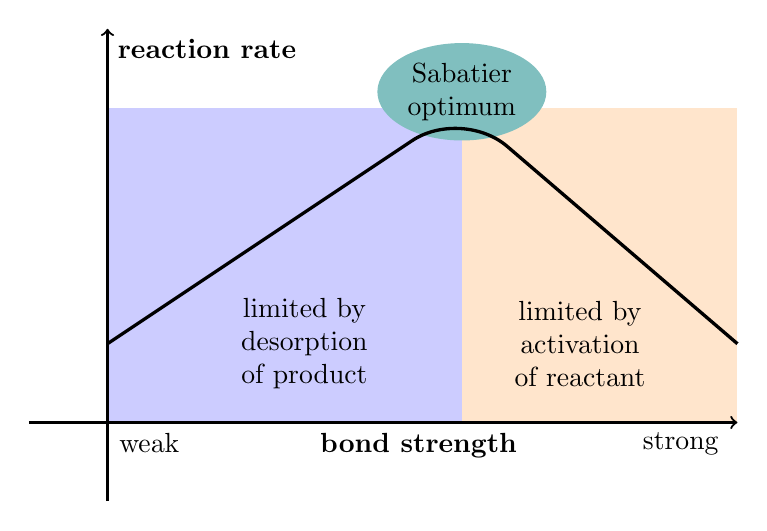
\begin{tikzpicture}[thick, align=center]

  \fill[blue!20] (0,0) rectangle (4.5,4);
  \fill[orange!20] (4.5,0) rectangle (8,4);
  \node at (2.5,1) {limited by\\desorption\\of product};
  \node at (6,1) {limited by\\activation\\of reactant};
  \node[ellipse, fill=teal!50, inner sep=2pt] at (4.5,4.2) {Sabatier\\optimum};
  \draw[->] (-1,0) -- (8,0) node[below, pos=0.17] {weak} node[below, pos=0.55, font=\bfseries] {bond strength} node[below, pos=0.92] {strong};
  \draw[->] (0,-1) -- (0,5) node[below right, font=\bfseries] {reaction rate};
  \draw[rounded corners=5ex, very thick] (0,1) -- (4.5,4) -- (8,1);

\end{tikzpicture}
\end{document}
